\section{Cortex}
\begin{frame}{Cortex}
\begin{justify}
            Cortex is a software project that complements and extends the capabilities of TheHive, a security incident response platform. It serves as an automation and orchestration engine. It automates the execution of various analysis tasks and security operations related to incident response by making api calls to various threat intelligence feeds and collects their outputs.
\end{justify}

\end{frame}

\subsection{Key Features}
\begin{frame}{Cortex: Key Features}
\begin{justify}
    \begin{enumerate}
    \item \begin{justify}
        \textbf{Automation:} Cortex allows users to define and execute a wide range of actions, such as analyzing observables, querying threat intelligence feeds such as VirusTotal, CyberCrime-Tracker etc. and interacting with other security tools and services.
    \end{justify}

    \item \begin{justify}
        \textbf{Analyzer Integration:} Cortex includes a collection of analyzers, which are plugins, enabled by adding API key, can be used to analyze different types of observables, for example, IP addresses, urls, hashes etc. These analyzers can be integrated into TheHive through Cortex and automatically perform tasks like malware analysis, DNS lookups etc. The generated reports can be shared with other security analysts of the organization which saves analysts time and standardize the investigation process.
    \end{justify}
\end{enumerate}
\end{justify}
\end{frame}
\begin{frame}{Cortex: Key Features continued}
    
\begin{enumerate}
 \setcounter{enumi}{2}

    \item \begin{justify}
        \textbf{Responder Integration:} Responders are plugins that can take action based on the analysis results. For example, if an analyzer detects a malicious URL, a responder can be configured to block the URL at the firewall or update an indicator of compromise blacklist.
    \end{justify}
    \item \begin{justify}
        \textbf{Extensibility:} Cortex allows organizations to develop custom analyzers and responders tailored to their specific needs. This flexibility makes it a valuable tool for organizations with unique security requirements.
    \end{justify}
    \item \begin{justify}
        \textbf{Integration with TheHive:} By integrating cortex with TheHive, it is easy to automate analysis and response actions into TheHive's case management and incident tracking workflows.
    \end{justify}
    
\end{enumerate}
\end{frame}

\subsection{Exploring the features}
\begin{frame}{Cortex Analzers}
\begin{justify}
    We have used a traning VM which have total 216 analyzers available and 16 of them are enabled with API key. To enable a new Analyzer, we just need to add the API key for that. A snapshot of some of the Analyzers from Cortex is shown below.
\end{justify}

\begin{figure}[htp]
    \centering
    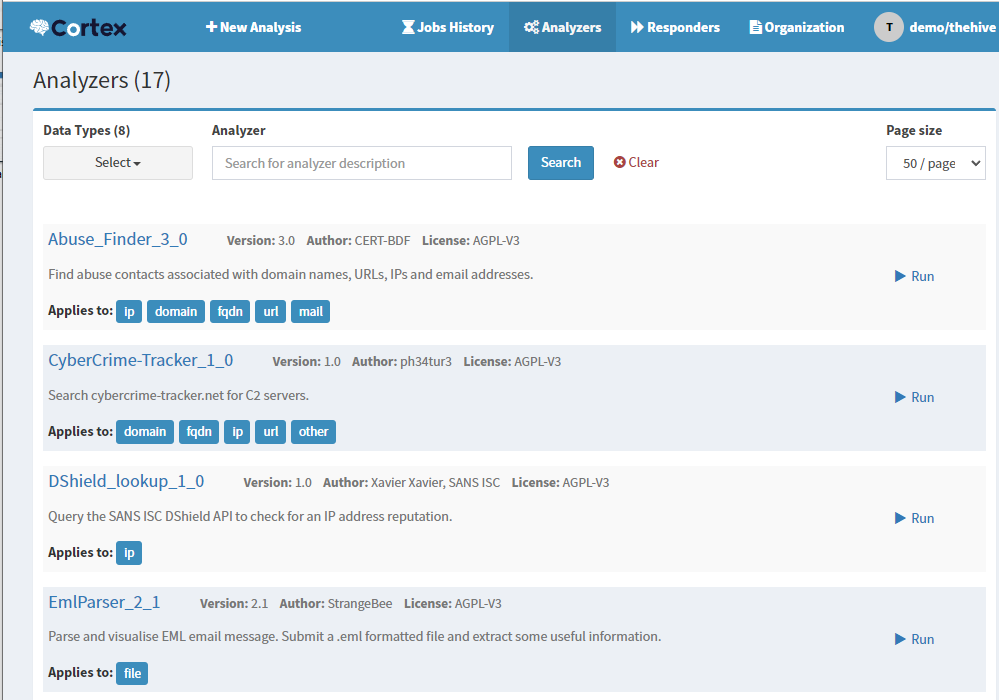
\includegraphics[scale = 0.28]{Cortex Analyzers.png}
    \caption{Cortex Analyzers}
    \label{fig:cortex-analyzers}
\end{figure}
    
\end{frame}

\begin{frame}{Enabling An Analyzer}
\begin{justify}
    In the \textbf{Organization} tab of Cortex, all the analyzers that are available are provided. To enable an analyzer, press the enable button.
\end{justify}
    \begin{figure}[htp]
    \centering
    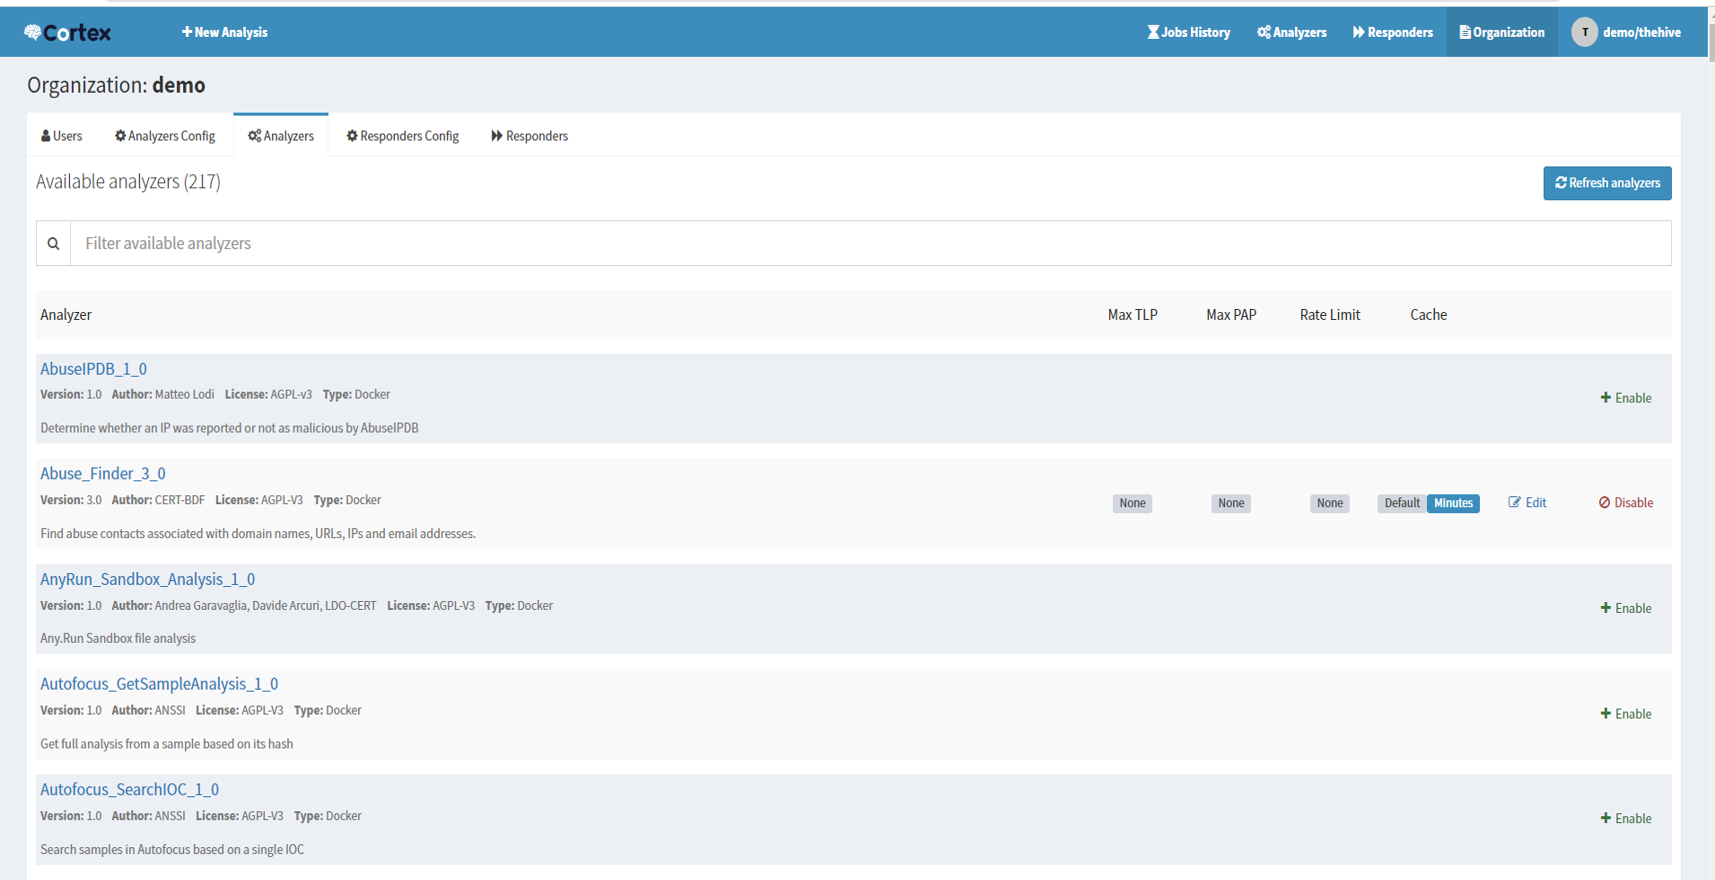
\includegraphics[scale = 0.35]{enabling an analyzer.png}
    \caption{Enabling an Analyzer}
    \label{fig:enabling-an-analyzer}
\end{figure}
\end{frame}

\begin{frame}{Enabling An Analyzer continued}
\begin{justify}
    The following box will be shown after pressing the enable button. To enable an analyzer, go to it's website and get the API key and put it here in the \textbf{key} option.
\end{justify} 

\begin{figure}[htp]
    \centering
    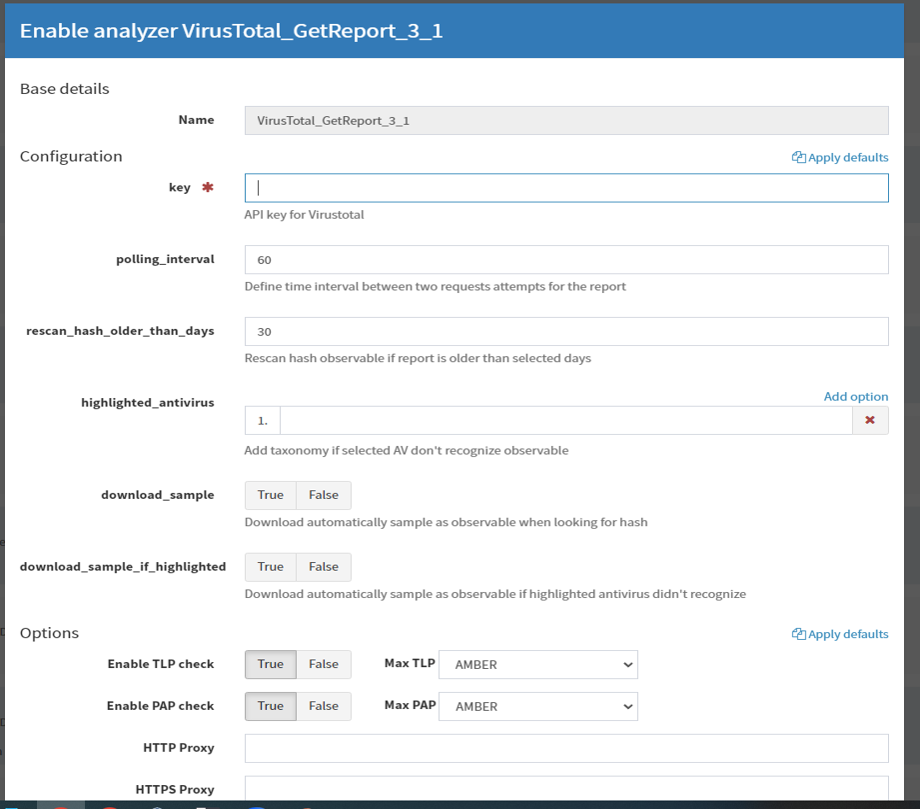
\includegraphics[scale = 0.35]{enabling an analyzer-2.png}
    \caption{Adding the API key}
    \label{fig:enabling-an-analyzer-2}
\end{figure}
    
\end{frame}

\begin{frame}{Running An Analyzer in Cortex}
\begin{justify}
    To run an analyzer, fill up the TLP, PAP, Data Type and Data and select the suitable analyzer accordingly. We can also select multiple analyzers for the same data.
\end{justify}

\begin{figure}[htp]
    \centering
    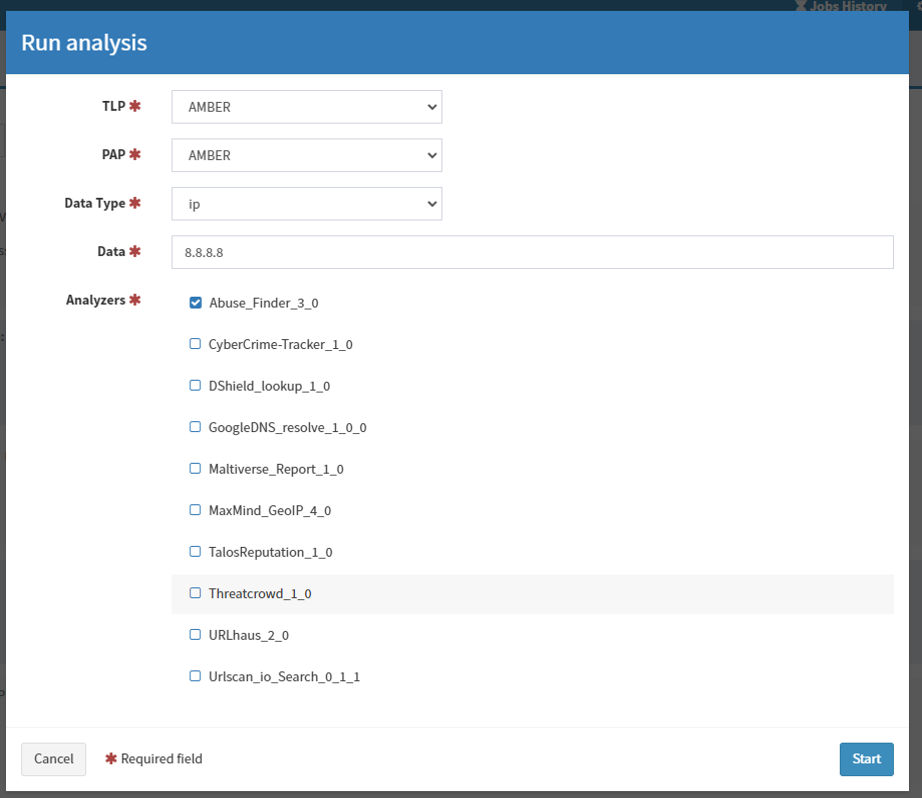
\includegraphics[scale = 0.35]{run-analyzer-cortex.png}
    \caption{Running an Analyzer}
    \label{fig:running-an-analyzer}
\end{figure}
    
\end{frame}

\begin{frame}{Running An Analyzer in Cortex continued}

\begin{justify}
    The running log can be seen from the \textbf{Jobs History} in Cortex. If the status is \textcolor{green}{\textbf{Success}}, then it has successfully generated report by querying into that analyzer. If the status is \textcolor{red}{\textbf{Failure}}, then there may be a problem in data type or format or the server may be down.
\end{justify}

\begin{figure}[htp]
    \centering
    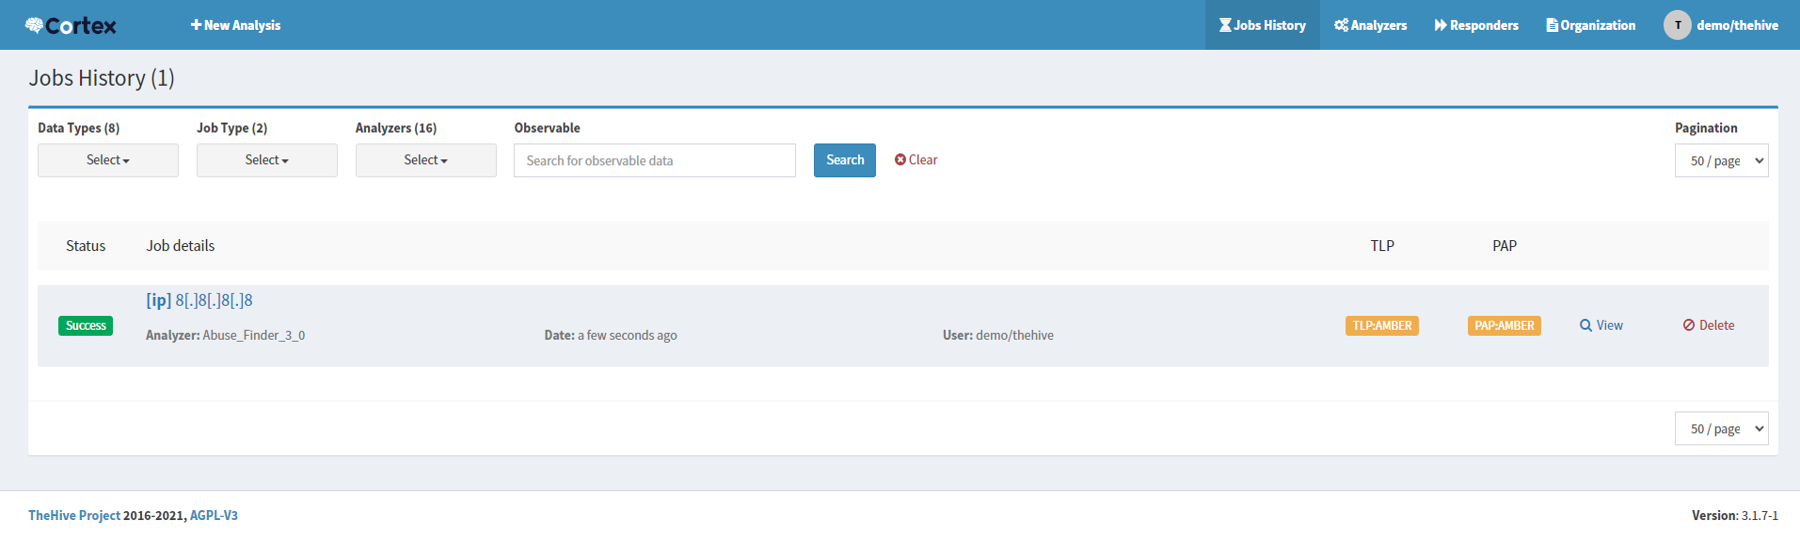
\includegraphics[scale = 0.35]{run-analyzer-cortex-2.png}
    \caption{Jobs history}
    \label{fig:running-an-analyzer-2}
\end{figure}
    
\end{frame}

\begin{frame}{Raw Report of Analyzer}

\begin{justify}
    By default in Cortex, the report generated by any analyzer is in JSON format which is not so human readable. 
\end{justify}

\begin{figure}[htp]
    \centering
    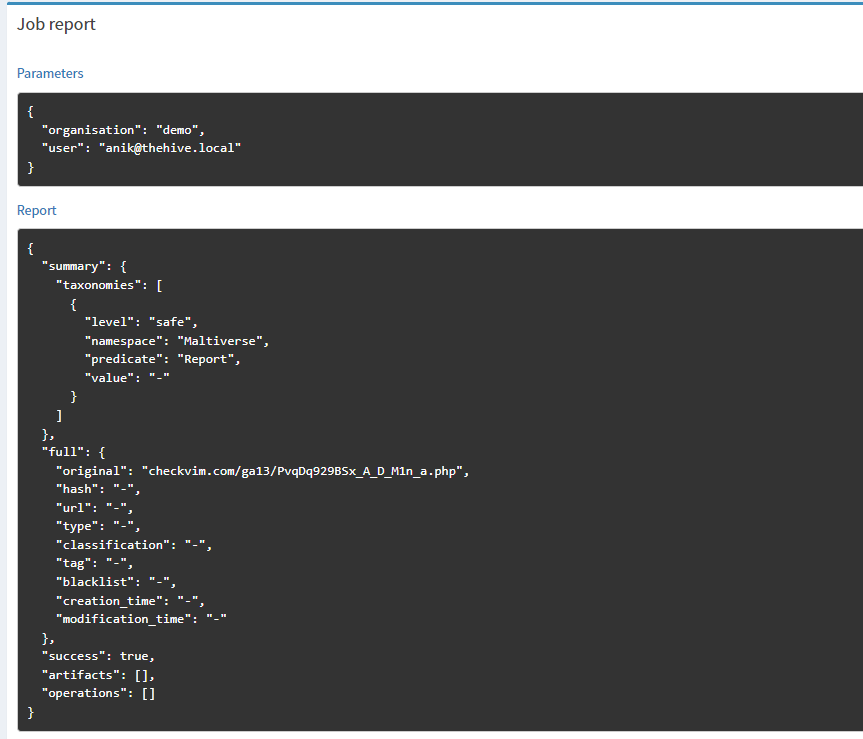
\includegraphics[scale = 0.25]{raw report.png}
    \caption{Raw report of the analyzer}
    \label{fig:raw-report}
\end{figure}
    
\end{frame}

\begin{frame}{Adding Templates From TheHive}
\begin{justify}
        To make the raw reports of Cortex more human readable, we can integrate the cortex with TheHive and add \textbf{templates} from admin account. In the traning vm, the cortex is integrated with TheHive. Therefore, we can analyze the observables from TheHive which will trigger the analyzer in Cortex.
\end{justify}

    \begin{figure}[htp]
    \centering
    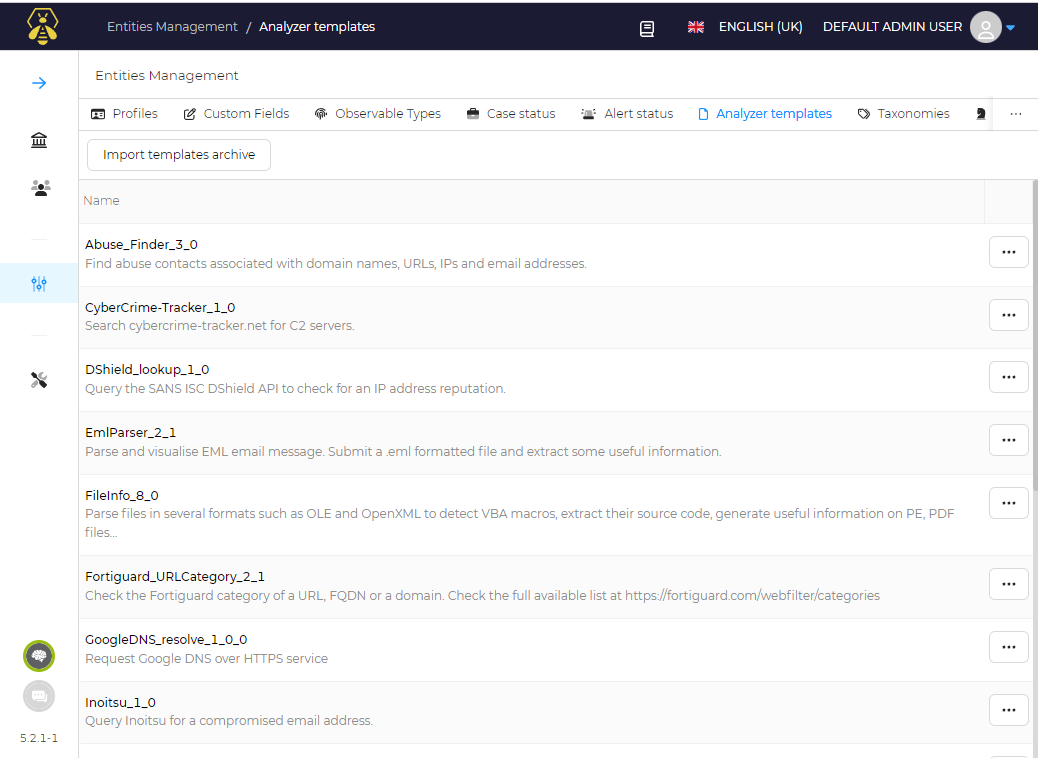
\includegraphics[scale = 0.22]{adding-templates.png}
    \caption{Adding Templates from TheHive's Admin}
    \label{fig:adding-templates}
\end{figure}
\end{frame}

\begin{frame}{Analyzing An Observable From TheHive}
\begin{justify}
    To analyze an observable from TheHive, we need to select an observable. Then among all the enabled analyzers, the ones that can analyze the selected data type will be shown. We can select one or more(up to all) analyzers and run which will then generate reports for the selected analyzers.
\end{justify}

\begin{figure}[htp]
    \centering
    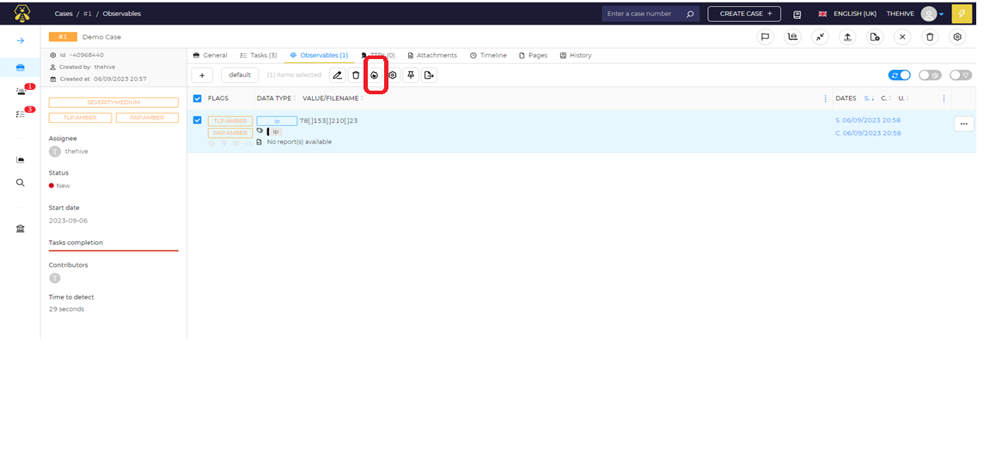
\includegraphics[scale = 0.37]{analyze-observables-1.png}
    \caption{Analyzing an observable from TheHive}
    \label{fig:analyzing-observable-1}
\end{figure}
    
\end{frame}

\begin{frame}{Analyzing An Observable From TheHive continued}
 \begin{figure}[htp]
    \centering
    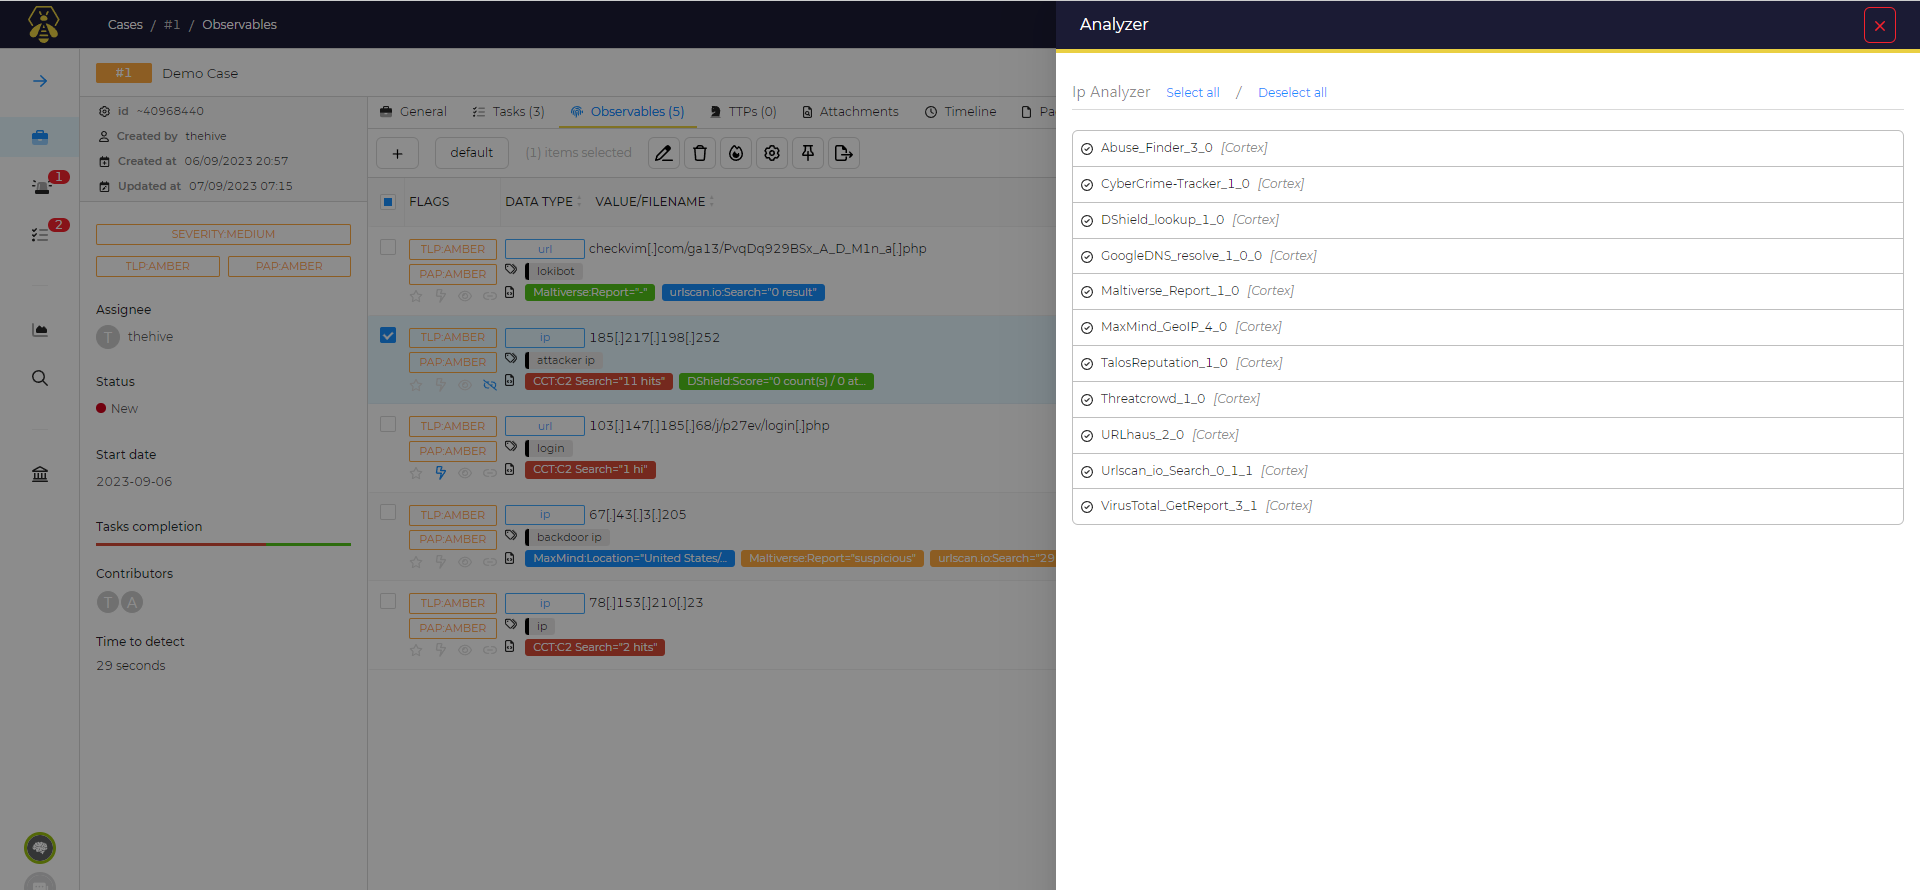
\includegraphics[scale = 0.27]{analyze-observables-2.png}
    \caption{Selecting the analyzer(s)}
    \label{fig:analyzing-observable-2}
\end{figure}   
\end{frame}

\begin{frame}{Analyzing An Observable From TheHive continued}
\begin{justify}
    Running an analyzer on an observable from TheHive automatically fires the analyzer from Cortex. The analysis report can be found in both Cortex and TheHive.
\end{justify}
 \begin{figure}[htp]
    \centering
    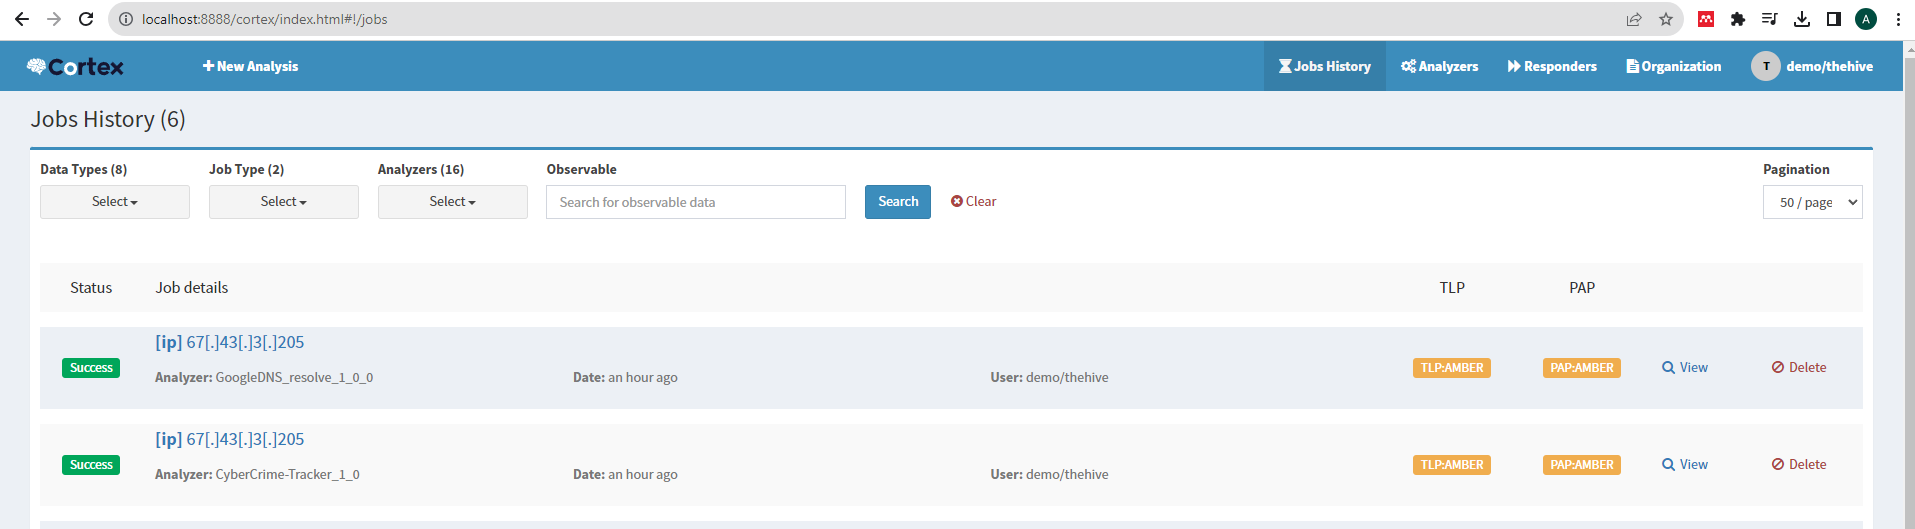
\includegraphics[width=1\textwidth]{analyze-observables-3.png}
    \caption{Running log of the analyzer}
    \label{fig:analyzing-observable-3}
\end{figure}
\end{frame}

\begin{frame}{Analyzer Report: VirusTotal}
\begin{justify}
    We have analyzed a malicious hash : \newline fb55414848281f804858ce188c3dc659d129e283bd62d58d34f6e6f568feab37 \newline which was collected from the VirusTotal website. By running the VirusTotal analyzer for this observable, we get the following report.
\end{justify}

 \begin{figure}[htp]
    \centering
    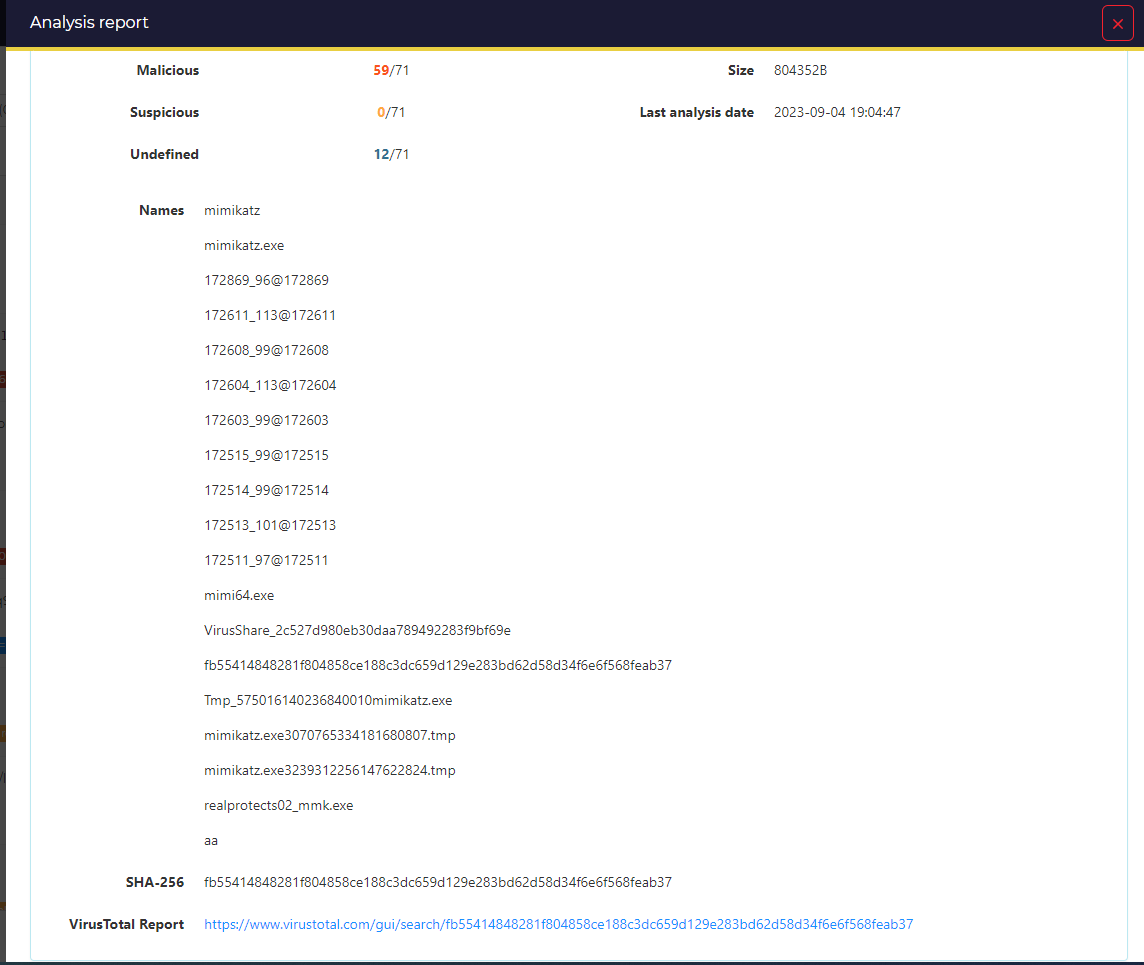
\includegraphics[scale=0.2]{virusTotal-1.png}
    \caption{VirusTotal Report}
    \label{fig:virusTotal-1}
\end{figure}
    
\end{frame}

\begin{frame}{Analyzer Report: VirusTotal continued}
 \begin{figure}[htp]
    \centering
    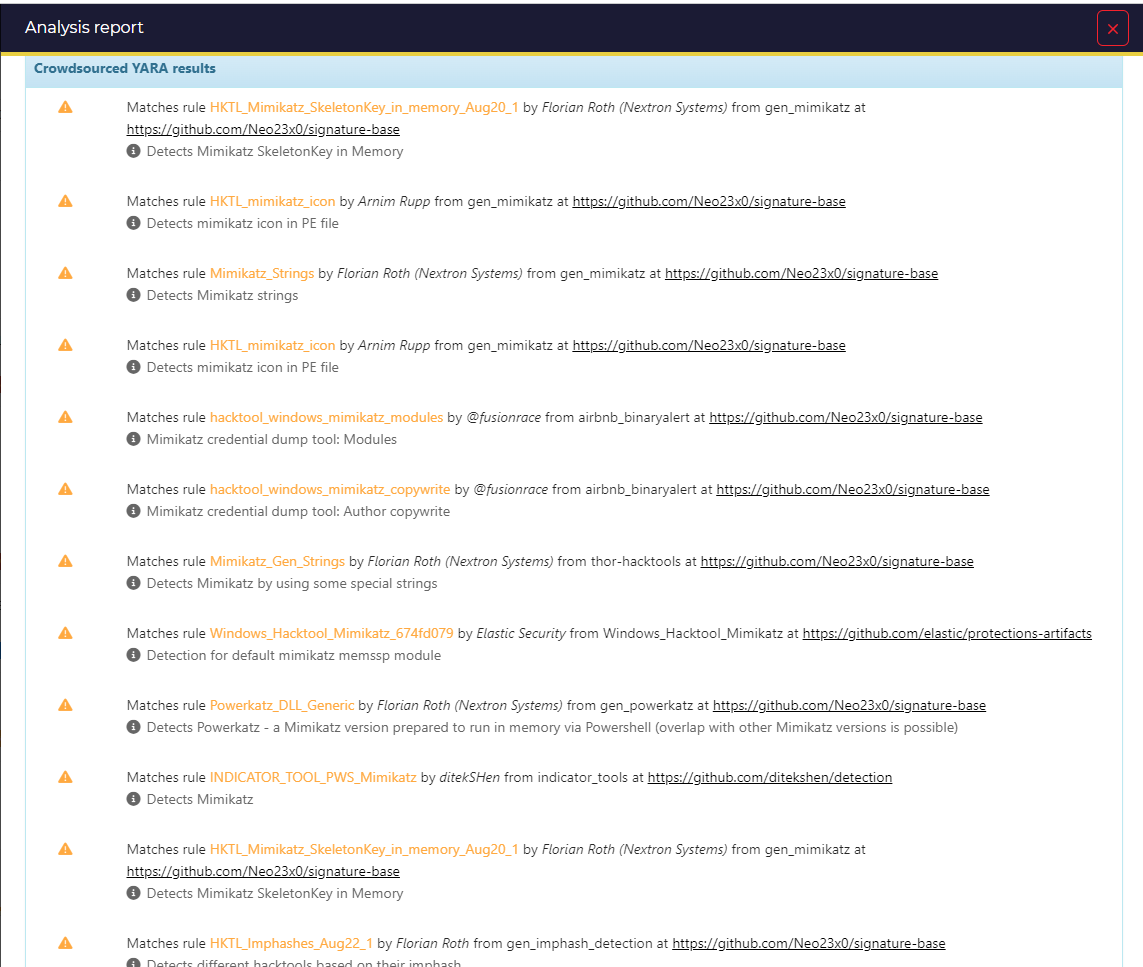
\includegraphics[scale=0.2]{virusTotal-2.png}
    \caption{VirusTotal Report}
    \label{fig:virusTotal-2}
\end{figure}
\end{frame}

\begin{frame}{Analyzer Report: VirusTotal continued}
 \begin{figure}[htp]
    \centering
    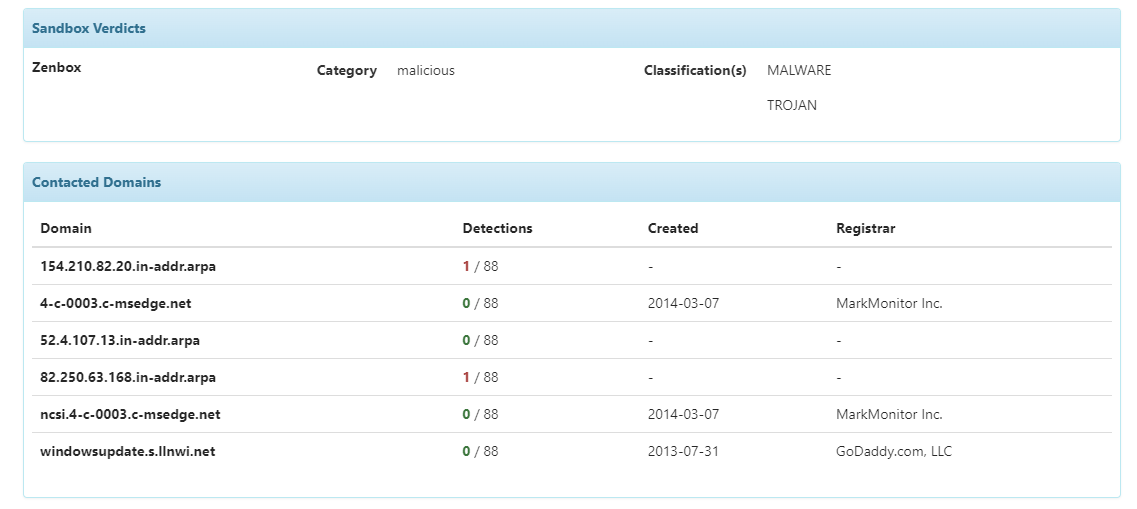
\includegraphics[scale=0.4]{virusTotal-3.png}
    \caption{VirusTotal Report}
    \label{fig:virusTotal-3}
\end{figure}

\end{frame}

\begin{frame}{Analyzer Report: VirusTotal continued}
 \begin{figure}[htp]
    \centering
    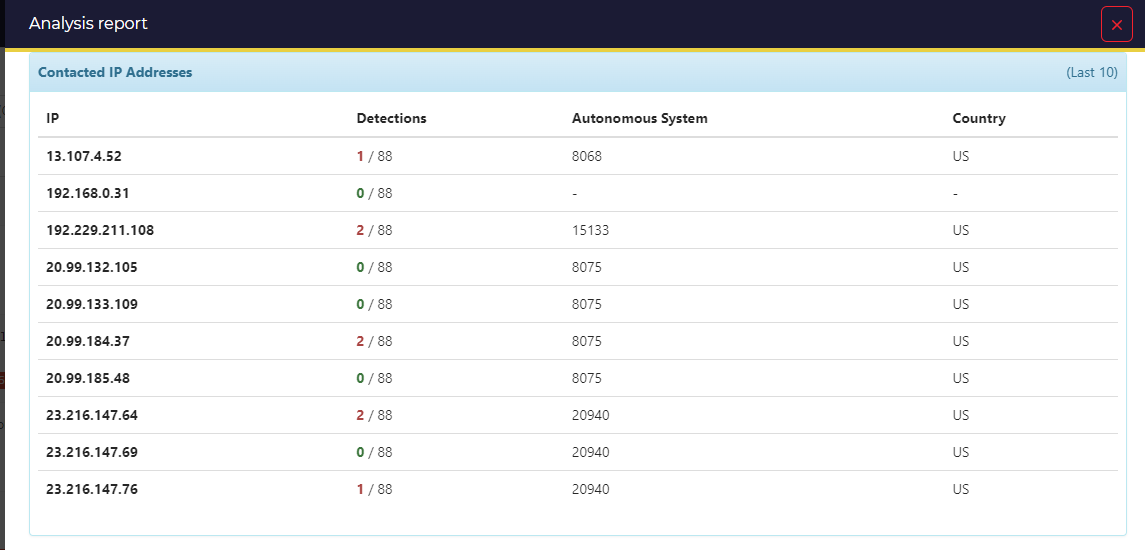
\includegraphics[scale=0.4]{virusTotal-4.png}
    \caption{VirusTotal Report}
    \label{fig:virusTotal-4}
\end{figure}

\end{frame}

\begin{frame}{Analyzer Report: VirusTotal continued}
\begin{justify}
    Here, it is showing the list of different security report website where some of them have already detected and marked this hash as malicious
\end{justify}
 \begin{figure}[htp]
    \centering
    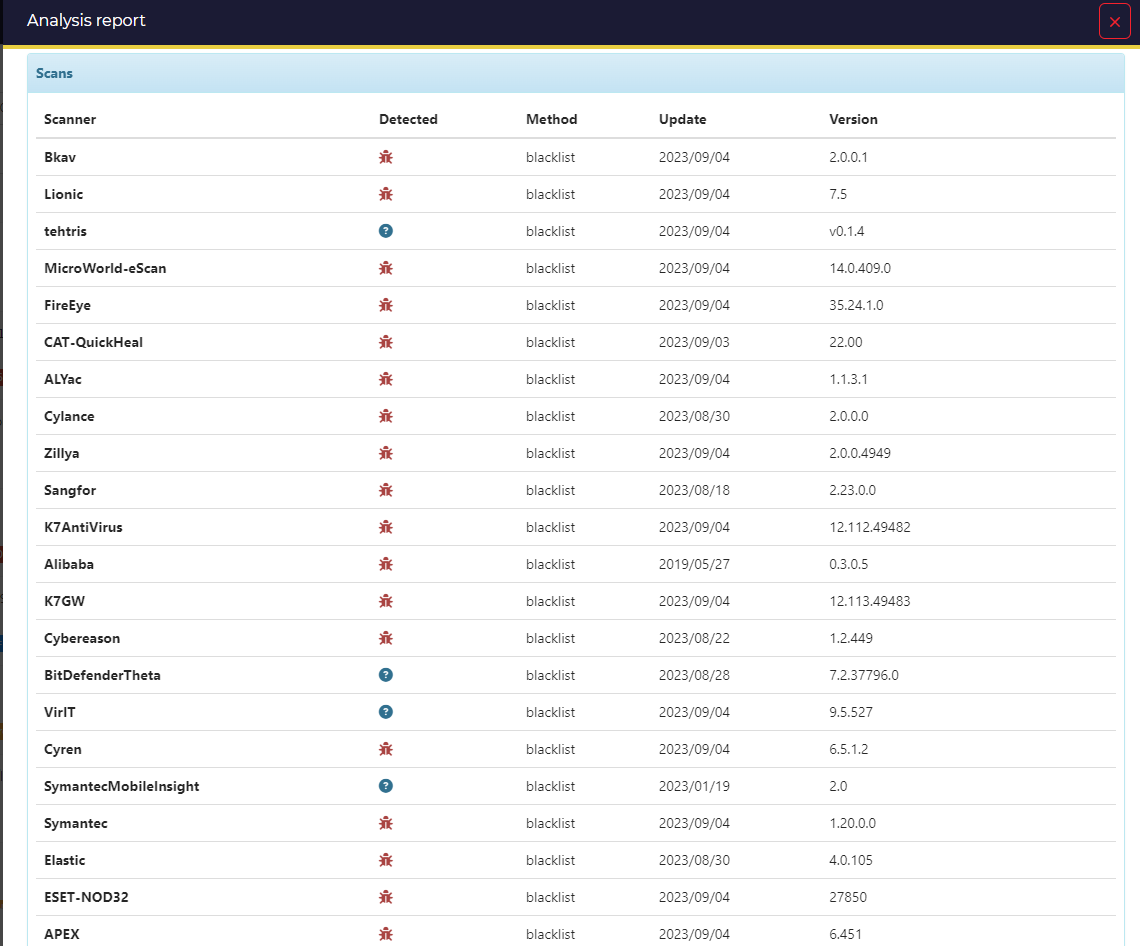
\includegraphics[scale=0.2]{virusTotal-5.png}
    \caption{VirusTotal Report}
    \label{fig:virusTotal-5}
\end{figure}

\end{frame}

\begin{frame}{Live Feed}
\begin{justify}
    The observables that are analyzed from TheHive via cortex can be seen by other analysts of the organization through Live Feed. If the analysis is done from Cortex, then it cannot be seen by other analysts. Thus, running analyzers from TheHive provides instant updates to all the analysts which help them to be up-to-date with the case progress.
\end{justify}

 \begin{figure}[htp]
    \centering
    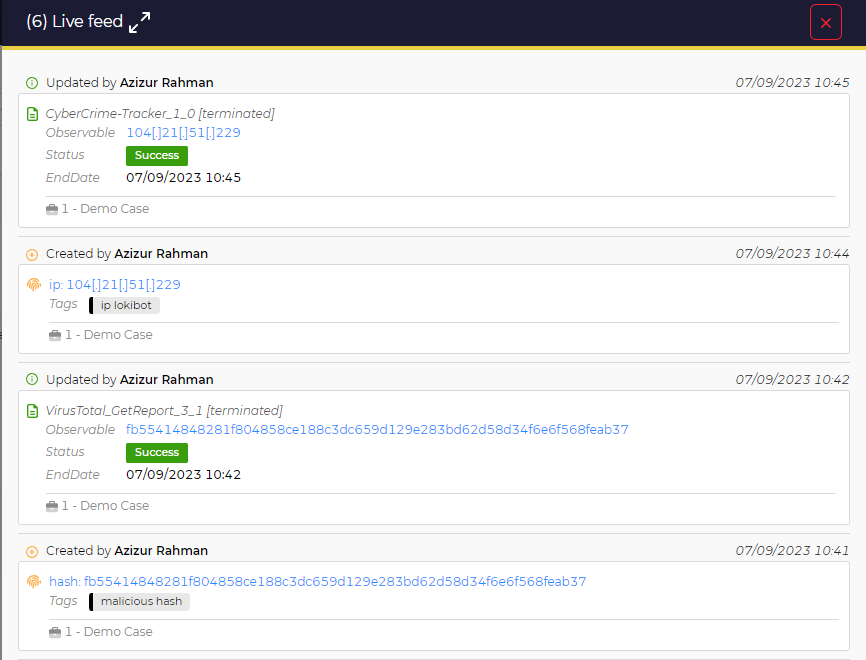
\includegraphics[width=0.5\textwidth]{live feed.PNG}
    \caption{Live Feed}
    \label{fig:livefeed}
\end{figure}
    
\end{frame}

\subsection{Conclusion}

\begin{frame}{Conclusion Remark}
\begin{justify}
    Cortex, integrated seamlessly into TheHive, empowers security professionals with a powerful arsenal of analyzers and responders, enhancing the platform's capabilities to detect, investigate, and respond to threats effectively. By harnessing the versatility and extensibility of Cortex, organizations can take their incident response to new heights, bolstering their cyber security posture in an ever-evolving threat landscape.As we wrap up our discussion on Cortex in TheHive, it is clear that this partnership is a game-changer for security teams, empowering them to detect, analyze, and mitigate threats more effectively than ever before.
\end{justify}
    
\end{frame}